\documentclass[11pt]{hmcpset}
\usepackage[margin=1in]{geometry}
\usepackage{amsmath,amssymb,enumerate,graphicx,url}

\newcommand{\ket}[1]{|#1\rangle}
\newcommand{\bra}[1]{\langle #1|}
\newcommand{\braket}[2]{\langle #1|#2\rangle}
\newcommand{\braketop}[3]{\langle #1| #2 | #3 \rangle}
\newcommand{\normsq}[1]{\left|#1\right|^2}
\newcommand{\prob}[2]{\normsq{\braket{#1}{#2}}}
\newcommand{\avg}[1]{\langle #1 \rangle}


\usepackage{xcolor}
\usepackage{listings}

\definecolor{mGreen}{rgb}{0,0.6,0}
\definecolor{mGray}{rgb}{0.5,0.5,0.5}
\definecolor{mPurple}{rgb}{0.58,0,0.82}
\definecolor{backgroundColour}{rgb}{0.95,0.95,0.92}

\lstdefinestyle{Python}
{
	language=Python,
	backgroundcolor=\color{backgroundColour},   
	commentstyle=\color{mGreen},
	keywordstyle=\color{magenta},
	numberstyle=\tiny\color{mGray},
	stringstyle=\color{mPurple},
	basicstyle=\footnotesize\ttfamily,
	breakatwhitespace=false,         
	breaklines=true,                 
	captionpos=b,                    
	keepspaces=true,                 
	%numbers=left,                    
	numbersep=5pt,                  
	showspaces=false,                
	showstringspaces=false,
	showtabs=false,                  
	tabsize=3
}



\name{}
\class{PHYS134}
\assignment{Homework/Project 8}
\duedate{2021-05-03}

\begin{document}
%\problemlist{}


%===========================================================
\begin{problem}[Blank Page]
	\begin{itemize}
		\item ... because for whatever reason \LaTeX \ insisted on putting the first problem on a new page even when I made it shorter and I just want to post this thing already.
	\end{itemize}
\end{problem}

\begin{solution}
	\vfill
\end{solution}
\pagebreak

%
%%===========================================================
%\begin{problem}[Diffraction]
%	\begin{enumerate}
%		\item Basic Fourier Transform stuff, including filtering images, throw out re/im, 
%		\item Use Fourier methods to propagate light through a circle, square, and edge
%		\item Lab: Fraunhoffer diffraction circular aperture linear stage
%		\item Lab: Fresnel diffraction with razor
%		\item Lab: Fraunhoffer diffraction with image analysis
%	\end{enumerate}
%\end{problem}
%
%\begin{solution}
%	\vfill
%\end{solution}
%\pagebreak


%===========================================================
\begin{problem}[2D Fourier Transforms (2D FFTs) in python]
	In this tutorial-style problem, you'll be asked to explore 2D fourier transforms and do image processing. First you'll load an image that you get from Sakai.
\begin{lstlisting}[style=Python]
img_rgb = imread("fourier3.jpg")
img_rgb.shape  # Note that this shape is NY,NX,3 for red,green,blue channels
\end{lstlisting}
Note that this is a 3-dimensional array whose last dimension selects the red, green, or blue channel. We'll treat it as a grayscale image and average the three channels together.
\begin{lstlisting}[style=Python]
img = mean(img_rgb,axis=-1)  # average across the last (color) axis
NY,NX = img.shape  # The first index, being the array's row, is Y, not X
imshow(img, cmap="gray")
\end{lstlisting}
Take the 2D fourier transform and shift it in both X and Y such that the zero frequency appears in the center of the array. Then plot the log of the magnitude of the frequency components.
\begin{lstlisting}[style=Python]
img_fft = fftshift(fft.fft2(img))
imshow(log(abs(img_fft)), cmap="gray")
\end{lstlisting}
Almost all image frequency spectra have a bright spot in the center because they contain no negative numbers. You can see some lighter structure on the top right and bottom left---the stripes in Fourier's jacket are made of sine waves along these directions.

This is a plot whose axes are labeled by pixel number, not spatial frequency. We'll use \texttt{fftfreq} again to get spatial frequencies. If you don't specify a pixel size, it assumes that each pixel is 1 unit on each side. This means that the maximum frequency is $\tfrac{1}{2}$ because a sine wave of that frequency would correspond to the highest-frequency pattern allowed---one that goes bright,dark,bright,dark... Since we have no pixel measurements, we can keep this default.
\begin{lstlisting}[style=Python]
xfreq = fftshift( fftfreq(NX,d=1.0) )  # NX frequencies in x direction; center 0
yfreq = fftshift( fftfreq(NY,d=1.0) )  # NY frequencies in y direction; center 0
extent_freq = (min(xfreq), max(xfreq), min(yfreq), max(yfreq))
imshow(log(abs(img_fft)), cmap="gray", aspect=NY/NX, extent=extent_freq)
\end{lstlisting}
I'd recommend using the \texttt{colorize} function from previous labs to see the phase of the frequency spectrum in addition to the magnitude.
\begin{lstlisting}[style=Python]
imshow(colorize(img_fft,log=True), aspect=NY/NX, extent=extent_freq)
\end{lstlisting}
You can get back the original image by doing the inverse shift and then inverse Fourier Transform. Because of rounding errors, you won't get back exactly the original image, but something very close plus a very small imaginary part. 
\begin{lstlisting}[style=Python]
almost = fft.ifft2(ifftshift(img_fft))
figure(figsize=figsize)
imshow(almost_original.real, cmap="gray")
\end{lstlisting}
The pixel values go from 0-255. What is the largest imaginary part and what is the largest difference between the original image and the inverse FFT?

The spectra are all symmetric across the origin (actually complex-conjugates) because the original image was real. The same applies to the Inverse Fourier Transform. If we keep only the real part of the spectrum and throw out the imaginary part, after we invert it, the result will be symmetric.
\begin{lstlisting}[style=Python]
keep_real_spectrum = fft.ifft2(ifftshift(img_fft.real))
imshow(colorize(keep_real_spectrum,log=True))
\end{lstlisting}
Do the same thing, keeping only the imaginary part, only the magnitude, and only the phase of the spectrum. The end of Lecture 24 should give you a hint about what to expect.

\end{problem}
\pagebreak


\begin{problem}[2D Fourier Transforms (2D FFTs) in python continued]
Now we're going to low-pass filter and high-pass filter this image. To do this, we make a 2D ``mask'' made of 1s for the spatial frequencies that we want to keep and 0s for the spatial frequencies we want to throw out.

\begin{lstlisting}[style=Python]
FX,FY = np.meshgrid(xfreq,yfreq)  # Two 2D arrays
mask = zeros((NY,NX))  # start the mask with all 0s
mask[(abs(FX)<=1/20)*(abs(FY)<=1/20)] = 1  # keep a square in the center
imshow(mask, cmap="gray", aspect=NY/NX, extent=extent_freq)
\end{lstlisting}
Show the masked frequency spectrum.  Note that $\log(0)$ is undefined, so it gives and error and shows up clear.
\begin{lstlisting}[style=Python]
imshow(log(abs(img_fft*mask)), cmap="gray", aspect=NY/NX, extent=extent_freq)
\end{lstlisting}
Now mask the frequency spectrum, invert the frequency shift, and finally invert the Fourier transform. Plot the resulting image back in pixel-space.
\begin{lstlisting}[style=Python]
filtered = fft.ifft2(ifftshift(img_fft*mask))  # * multiplies pixel by pixel
imshow(filtered.real, cmap="gray")
\end{lstlisting}
As long as you do things symmetrically to the frequency spectrum, the inverted Fourier transform will stay real up to rounding errors. To high-pass, just invert the mask.
\begin{lstlisting}[style=Python]
highpass_mask = 1-mask
filtered = fft.ifft2(ifftshift(img_fft*highpass_mask))
imshow(filtered.real, cmap="gray")
\end{lstlisting}

\begin{enumerate}
	\item Find some other image and high-pass or low-pass filter it.
	\item Create a new 256x256 array (image) that's all zeros except for a small square within around 8 pixels of the the origin, which is ones. Show the colorized fft. If your small square is in the center of the array rather than at the corner, don't forget to \texttt{fftshift} it.
	\item Same, but for a small circle of radius around 32 pixels.
	\item Same, but for a gaussian. It might help to set log=False in colorize.
\end{enumerate}





\end{problem}
\pagebreak



%===========================================================

\begin{problem}[2D Diffraction Fit]
	We're going to analyze the diffraction pattern that I captured directly on the camera's sensor (no lens) as shown below. I had to capture the picture in the camera's RAW mode, since display formats like JPG have values that are not linear in intensity.
	
	\vspace{-1em}
	\begin{center}
		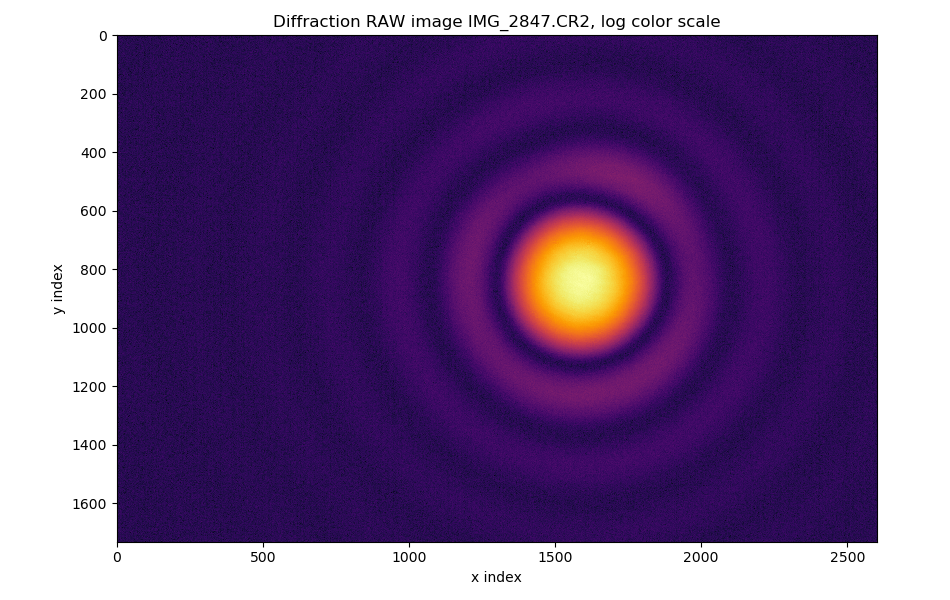
\includegraphics[width=0.70\textwidth]{diffraction2D_whole_image_log.png}
	\end{center}
	\vspace{-1em}

	It would be great to fit the whole pattern, but because the laser isn't completely uniform, students have only ever had success fitting the central peak. I've cropped out the central 400x400 as a numpy array, which you can download and load using the command \texttt{img = load("Lab7DiffractionCenter.npy")}. With the slightly different color scale, you can see some ugly features that don't look like random noise. If we tried to do a 2D fit, how would we assign errors to each pixel value? If I took 5 pictures, they would each exhibit the same ugly pattern. We'll fix both problems by taking averages and standard deviations in thin rings around the center. The center didn't quite align with a pixel and is located at \texttt{(cx, cy) = (199.9, 199.3)}.

	\vspace{-1em}
	\begin{center}
		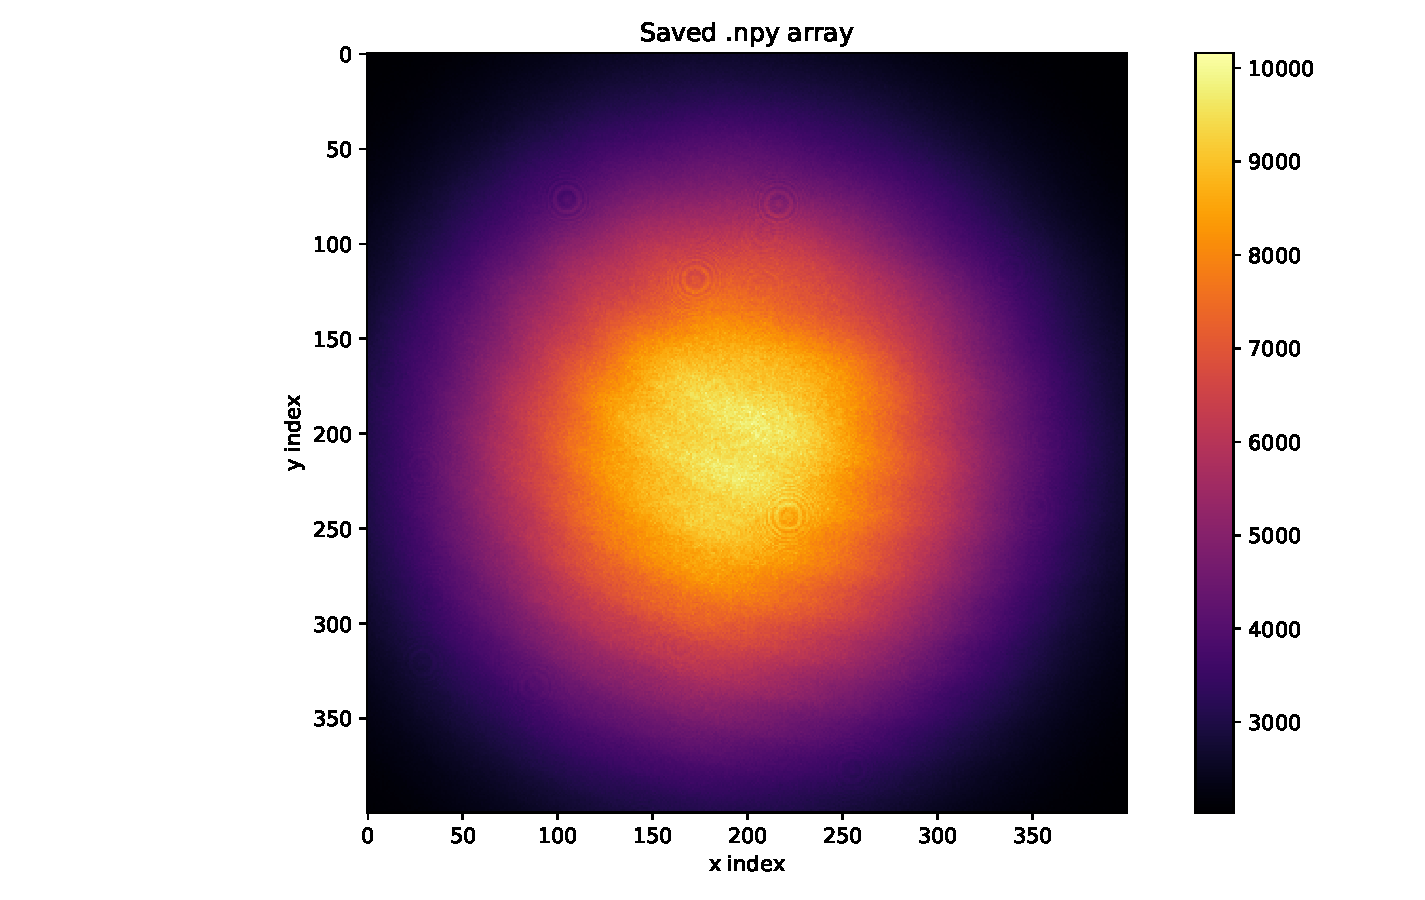
\includegraphics[width=0.50\textwidth]{diffraction2D_saved_array.pdf}
	\end{center}
	\vspace{-1em}
	
	The first step is to set up your 2D coordinate information and calculate the distance of each pixel from the center.
\begin{lstlisting}[style=Python]
# 2D coordinates
xaxis = arange(img.shape[1])
yaxis = arange(img.shape[0])
X,Y = meshgrid(xaxis,yaxis) # 2D arrays of X and Y coordinates

# Make a 2D array representing radius from center in number of pixels
R = sqrt( (X-cx)**2 + (Y-cy)**2 ) 
\end{lstlisting}
\end{problem}
\pagebreak







%===========================================================
\begin{problem}[2D Diffraction Fit (cont)]

The next step is to bin the data into rings of some width. Then you find the average value in each ring and the standard error of all of those values. I was going to let you each figure this out yourselves, but here is a suggestion:
\begin{lstlisting}[style=Python]
ringwidth= 2 # 2 pixel wide bins. Doesn't have to be interger
BIN = np.round(R/ringwidth).astype(int)  # 2D array of bin number for each pixel

# make rings out to the closest edge, not all the way to the corners
nbins = np.min([BIN[0,:], BIN[-1,:],BIN[:,0], BIN[:,-1]]) # =100 here

# Make empty arrays to save what we need, bin by bin
count  = zeros(nbins)
radius = zeros(nbins)
means  = zeros(nbins)
stds   = zeros(nbins)
for i in range(nbins):   # For each bin, save:
	count[i]  =  np.sum(     BIN==i ) # number of pixels with this bin number
	radius[i] =  np.mean(  R[BIN==i]) # mean radii of each ring
	means[i]  =  np.mean(img[BIN==i]) # mean pixel value in each ring
	stds[i]   =  np.std( img[BIN==i], ddof=1) # std pixel value
\end{lstlisting}

Check that the number of pixels in each ring grows linearly with radius and the width of the bin. The \texttt{count} array should be roughly \texttt{2*pi*radius*ringwidth}.

Now we have all that we need to do a 1D fit:

\begin{lstlisting}[style=Python]
xdata = radius  # radius of each ring in number of pixels
ydata = means   # mean pixel value in that ring
yerr  = stds/sqrt(count)  # standard error of those means
\end{lstlisting}

The theoretical prediction for the intensity (without accounting for uniform background light) is
\[
I(\alpha) = 4 I_{max} \frac{J_1(\alpha)^2}{\alpha^2}
\]
where $J_\nu(\alpha)$ is a Bessel function. Python can numerically compute this:
\begin{lstlisting}[style=Python]
from scipy.special import jv
jv(1,alpha)
\end{lstlisting}
The dimensionless parameter $\alpha = ka \sin{\theta}$, where $k=2\pi/\lambda$, $\lambda$=632.8\,nm, $a$ is the radius (not diameter) of the small circular aperture (``hole'') that you are fitting for, and $\theta$ is the angle that each pixel makes from the center of the aperture. To know $\theta$, you need to know that the pixel spacing in my camera is 8.58\,$\mu$m, and that the camera was 60\,cm away from the aperture. Sketch a picture of what you need to calculate $\theta$ for each pixel.

Despite the non-random looking noise, averaging around rings seems to have done a reasonable job of averaging out the ripples and the dust specs on the sensor. Since the ripples and dust specs are uncorrelated with the pattern we are measuring, averaging enough of them together acts like random noise.

\begin{itemize}
	\item Show all three usual plots: data and fit, residuals, normalized residuals.
	\item Calculate all of the usual things: $\chi^2$, $\chi^2$/dof, and PTE. I got a pretty good PTE with this image.
\end{itemize}

\end{problem}
\pagebreak




\end{document}
